\section{Executive Summary}
\begin{figure}[]
\centering
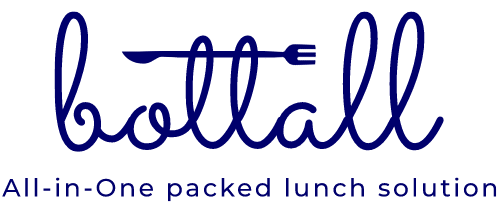
\includegraphics[width=0.5\textwidth]{logo.PNG}
\end{figure}

A bottle for food and drinks in a single ALL-IN-1 solution through two divisible sections, so you can have a full meal in any place without the need to carry two different containers. The steel bottle is airtight and the two sections (the lower for the food, the upper for the drink) are thermally insulated, with the possibility of heating the food inside through a simple USB port. A dedicated app for smartphones, via bluetooth, allows you to monitor the temperature during heating and to receive news and curiosities of various kinds on health, recipes or reminders on hydration. Capacity 0.45l for food, 0.5l for drink.
\subsection{Company Description}
BottAll team is made up of five founders, engineers with electrical energy and computer knowledges with a great desire to get involved.
\subsection{Industry Analysis}
BottAll will compete in the food and beverage storage container industries. The industry is in the growing phase of its life cycle. Growth is being driven by a lot of factors but primarily the increased awareness of the importance of environmental pollution and the attention to what we eat (talking about healthy food trend). At the moment the value of this Industry reaches 8.75 USD Billion for reusable water bottles and nearly 4 USD Billion for lunch boxes. 
 
\subsection{Market Analysis} 
According to the data found in [1] we were able to identify our market segment. We found our customers in people who decide to stay out during the break to have lunch and eat food prepared at home. There are several possible competitors which use different shape, material and styles to create their products but no one have a 2in1 solution to store both food and drink and no one use electronics inside the storage container to warm up the food. 

\subsection{Marketing Plan}
Our goal is to sell the whole product: both water bottle and food container in the same package, but we do not neglect the possibility to buy them separately. BottAll will be sold mainly through our online shop but will be also present in home goods stores such as Zara Home and Maison du Monde.

\subsection{Operations and Development Plan}
BottAll will be designed and improved in the R\&D of our society and then it will be manufactured by our partner companies. Our main business strategy is to subcontract all the production of basic pieces to some partner company in order to maintain costs sufficiently low since the beginning. So, we will assembly manufactured components. In future years maybe we will expand, and we will produce our own components indoors.

\subsection{Financial Projection and funding sought}
The first period will be devoted to the design of the product and to set up the structure of the company, and after we will prototype and test. Our following step will be to conduct a campaign of crowdfunding. The objective of our society is to be fully operative by the end of 2021. According to our financial forecasts, our industry will become financially independent in 3 years.

 